% !TEX root = ../mat999.tex
\newpage
\section{Expectation}
Recall that a RV is a measurable function $X:(\Omega, \F)\mapsto (\bar{\R}, \bar{\B})$
\begin{dfn}[Expectation] The expectation (expected value/ mean) of RV $X$ defined on the probability space $(\Omega, \F, \prob)$ is \begin{equation*}
    \E(X) := \into X d\prob
\end{equation*}
Provided the integral is well-defined. \\
\textbf{Note:} $\E(X)$ is well-defined iff $\min(\E(X^+), \E(X^-)) < \infty$
\end{dfn}
Recall that for a RV X defined on $(\Omega, \F, \prob)$, we define $\mu_X$ the probability measure induced by $X$ on $(\bar{R}, \bar{\B})$ (push forward of $\prob$ under map $X$)
\begin{equation*}
    \mu_X(B) := \prob(\{\omega| X(\omega) \in B\}) \quad \forall B \in \bar{\B}
\end{equation*}

\begin{dfn}
    A RV $X$ on $(\Omega, \F, \prob)$ is \textbf{discrete} if $\exists \{x_k\} \subset \bar{\R} \text{ be countable}, x_k \neq x_l \text{ for } k\neq l$ s.t.
    \begin{align*}
        &\prob(X=x_k) = \mu_X(\{x_k\}) > 0 \\
        &\bigs{k} \prob(X=x_k) = \bigs{k}\mu_X(\{x_k\}) = 1
    \end{align*}
\end{dfn}we denote by $p(x) := \mu_X(x)$ the probability mass function of the RV X. The set $\{x|p(x)>0\}$ is called the support of the pmf of $\mu_X$
\begin{prop}
For a discrete RV $X$ with support $\{x_k\}$
\begin{enumerate}
    \item $\E(X)$ is defined $\Longleftrightarrow \min\{\bigs{k:x_k>0}x_kp(x_k),-\bigs{k:x_k<0}x_kp(x_k)\} < \infty$
    \item If $\E(X)$ is defined then 
    \begin{equation*}
        \E(X) = \bigs{k}x_kp(x_k)
    \end{equation*}
    \item $X\in \ls{1} \Longleftrightarrow \E(\abs{X})<\infty \Longleftrightarrow \bigs{k}\abs{x_k}p(x_k) < \infty$
    \item For any measurable function, $h: \bar{\R} \mapsto \bar{\R}$ the RV $Y = h(X)$ is discrete and 1-3 hold with $Y$ and $h(x_k)$
\end{enumerate}
\end{prop}
\begin{example}
If $h(x) = \sin(x)$ then $\E(\sin(X)) = \bigs{x} \sin(x_k) p(x_k)$ if expectation for $X$ is well-defined
\end{example}
\pf First ignore the zero measure part:  Let $A_k:=X^{-1}(x_k) = \{\omega|X(\omega) = x_k\} $ and $X' := \bigs{k}x_k \I_{A_k}$ \\
Then $X'$ is a discrete RV and $X = X'$ a.s. Assume first $X \geq0$ a.e. $\implies X' \geq 0$ a.e. and we have the integral are equal:
\begin{equation*}
    \E(X) = \E(X') = \int \bigs{k}x_k \I_{A_k}d\prob
\end{equation*}
Let $X_n := \bigs{k=1}^n x_k \I_{A_k}, X_n\uparrow X'$ and by MCT:
\begin{align*}
    \E(X) &= \E(X') = \int X' d\prob = \int \biglim{n} X_n d\prob = \biglim{n} \int X_n d\prob = \biglim{n} \bigs{k=1}^n x_k \prob(A_k) = \bigs{k} x_k \prob(A_k)\\
    \E(X) &= \bigs{k} x_k \prob(A_k)
\end{align*}\qed
\newpage 
\begin{dfn}AC and pmf \\
    The probability measure induced by RV $X, \mu_X$ is \textbf{absolutely continuous (AC)} w.r.t Lebesgue's measure $\lambda$, if $\mu_X(\R) = 1$ and if $\exists f:(\R, \B) \mapsto ([0,\infty), \B)$ measurable s.t. 
    \begin{equation*}
        \forall B \in \B, \prob(X\in B) = \mu_X(B) = \int_B fd\lambda = \int_\R f \I_B d\lambda
    \end{equation*}f is called the \textbf{density} of induced measure $\mu_X$
\end{dfn}
\begin{thm}[Change of variables formula]
\label{change}
Let $X$ be a RV on $(\Omega, \F, \prob)$ and induced measure $\mu_X$ be distribution of X
\begin{enumerate}
    \item suppose that $h: (\bar{\R}, \bar{\B})\mapsto (\bar{R}^+, \bar{\B}^+)$ is measurable,let $Y:=h(X)$ Then $Y$ is non-negative RV with
    \begin{equation*}
        \E(Y) = \int Y\diff\prob = \int h(X) \diff\prob  = \int_{\bar{\R}} h \diff\mu_X
    \end{equation*}
    \item If $h: (\bar{\R}, \bar{\B})\mapsto (\bar{\R}, \bar{\B})$ is measurable then for $Y = h(X)$
        \begin{enumerate}
            \item $\E(Y) = \int Y\diff \prob$ is defined iff $\int h \diff\mu_X$ is defined and then
            \begin{equation*}
                \E(Y) = \int h \diff \mu_X
            \end{equation*}
            \item $Y\in \ls{1}(\Omega,\F, \prob)$ iff $h\in \ls{1}(\bar{\R}, \bar{\B}, \mu_X)$
        \end{enumerate}
    \begin{rem}
    Part 1 and 2 holds for any RVs (discrete/ continuous/ singular ...)
    \end{rem}
    \item If $X$ has a density $f$ ,then 
    \begin{equation*}
        \E(Y) = \int_\R hf \diff\lambda
    \end{equation*}(Lebesgue integral) with $\E(Y)$ is defined iff $\int_\R hf \diff\lambda$ exists

    \item If $X$ has density $f$ and $h: \R \mapsto \R^+$ is measurable s.t. $g(x):= h(x)\cdot f(x)$ is Riemann integrable on any finite interval, then 
    \begin{equation*}
        \E(Y) = \int_\R fh \diff\lambda = \inti h(x)f(x) \diff x
    \end{equation*}
    \item Condition on $h$ in 4 and we generalise it to the case $\R \mapsto \R$ \\
    $\E(Y)$ is well-defined if $\min\{\inti h^+f(x) \diff x, \inti h^-f(x) \diff x\}<\infty$ and then we have:
    \begin{equation*}
        \E(Y) = \inti h(x)f(x) \diff x
    \end{equation*}
\end{enumerate}
\end{thm}
\pf 

\newpage
\begin{cor}
$X\in \ls{1}$ iff $\inti \abs{x}f(x) \diff x < \infty$
\end{cor}
\begin{cor}
If $X$ has a density $f$ s.t. $g(x)= xf(x)$ is Riemann integrable on any finite interval, then $E(X)$ is defined iff
\begin{equation*}
    \int_{-\infty}^0 x f(x) \diff x > -\infty \quad\text{or}\quad \int_{0}^\infty x f(x) \diff x < \infty
\end{equation*} and if defined then
\begin{equation*}
    \E(X) = \inti xf(x) \diff x
\end{equation*}
\end{cor}
\begin{rem}
This definition does not means the expectation is finite, only existence can be guaranteed
\end{rem}
\begin{prop}
Let $X_1, X_2$ be RVs on $(\Omega, \F, \prob)$
\begin{enumerate}
    \item If $X_n$ are uniformly bounded $(\abs{X_n}\leq c < \infty \quad a.s).$ and $X_n \rightarrow X$ a.s. then $X_n \rightarrow X$ in $\ls{1}$ \\
    Bounded Convergence Theorem
    \item If $X_i \in \ls{1}$ then $\E(\bigs{i=1}^n X_i) = \bigs{i=1}^n \E(X_i)$
    \item If $X\geq 0 $ a.s. then $\E(X) \geq 0$. Also if $X_i\geq 0$ a.s. $\E(\bigs{i=1}^\infty X_i) = \bigs{i=1}^\infty \E(X_i)$, this is always well defined
    \item If $\E(X) < \infty$ then $\prob(X < \infty ) = 1$
    \item If $X_n \geq 0$ a.s. and $\bigs{n=1}^\infty \E(X_n) < \infty$ then by 4, $\bigs{n=1}^\infty X_n < \infty$ a.s. and in particular, $X_n\xrightarrow{a.s.}0$
\end{enumerate}
\end{prop}
\newpage
\begin{prop}
Suppose $X$ is a measurable function defined on $(\Omega,\F, \mu)$ with $\mu(\Omega)<\infty$ Then
\begin{enumerate}
    \item if $X\in \ls{p}$ for $p\geq1$ then $X\in \ls{r}$ for $r \in [1,p]$ (i.e. $\ls{p}$ spaces are nested and it is not necessarily the case for infinite measure)
    \item If $\mu = \prob$, then $\norm{X}_r \leq \norm{X}_p$, for $p \geq r \geq 1$, that is existence of higher moment always imply existence of lower moment.
\end{enumerate}
\end{prop}
\pf If $p >1$ and $r\in [1,p)$, define $p' = \frac{p}{r} > 1$ then $\exists q' > 1 \quad \frac{1}{p'} + \frac{1}{q'} = 1$ Conjugate. and then we have (By Holder's inequality \ref{holder}):
\begin{align*}
    \norm{X}_r^r = \int \abs{X}^r \cdot 1 \diff\mu &\leq  \left(\int \abs{X}^{rp'}  \diff\mu\right)^{\frac{1}{p'}}\left(\int \abs{1}^{q'}  d\mu\right)^{\frac{1}{q'}} \\
    &=\left(\int \abs{X}^p \diff\mu\right)^{\frac{r}{p}}\mu(\Omega)^\frac{1}{q'} \\
    &= \norm{X}_p^r\mu(\Omega)^\frac{1}{q'} \\
    \implies \norm{X}_r &\leq  \norm{X}_p \mu(\Omega)^\frac{1}{rq'} \leq \infty
\end{align*}\qed
\newpage
\subsubsection*{convex function and Jensen's inequality}
\begin{figure}[h]
    \centering
    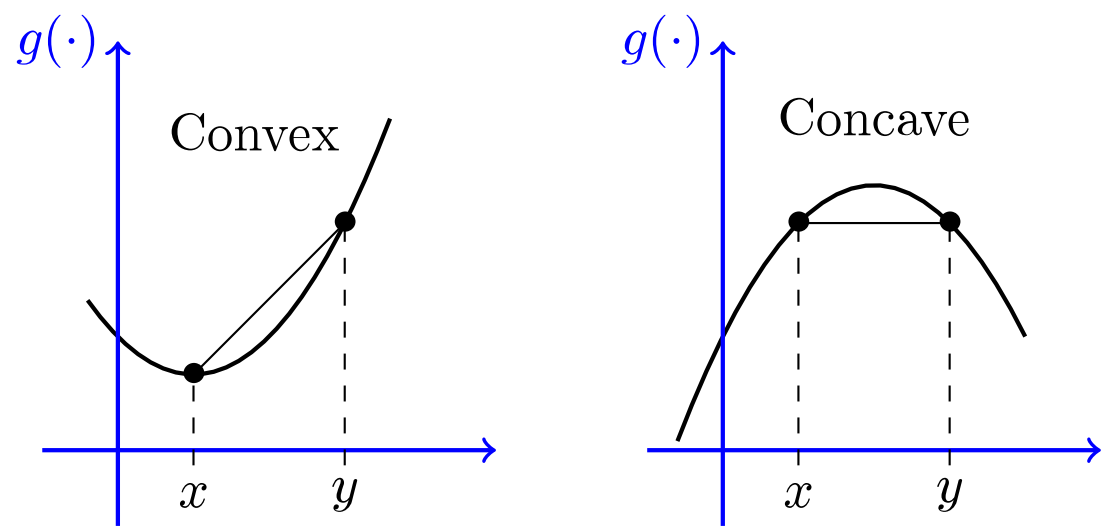
\includegraphics[scale = 0.2]{convex.png}
    \caption{Convex and concave function}
\end{figure}
\begin{dfn}[Convex function] A function $\phi: I \mapsto \R$ is convex on an open interval $I$ if $\forall x,y \in I$ and parameterise by $t\in(0,1):$
\begin{equation*}
    \phi(tx + (1-t)y)\leq t\phi(x) + (1-t)\phi(y), \quad \forall t \in (0,1)
\end{equation*}
\end{dfn}
\begin{lem}[Slope inequality]If $a < b < c \in I$ then we have \\
(Notation: $S([a,b]) := \frac{\phi(b) - \phi(a)}{b-a}$)
\begin{align*}
    &\frac{\phi(b) - \phi(a)}{b-a} \leq \frac{\phi(c) - \phi(a)}{c-a} \leq \frac{\phi(c) - \phi(b)}{c-b}   \\
    &S([a,b]) \leq S([a,c]) \leq S([b,c])
\end{align*}
\end{lem} Consider slope of the triangle formed by a,b,c:
\vspace{3cm}
\begin{cor}
Given convex function $\phi$, For any $x \in I$ left and right derivatives $D_{-\phi}$ and $D_{+\phi}$ exist and satisfy:
\begin{align*}
    D_{-\phi} := \biglim{h\rightarrow 0^+} \frac{\phi(x) - \phi(x-h)}{h} \leq \biglim{h\rightarrow 0^+} \frac{\phi(x+h) - \phi(x)}{h} =: D_{+\phi}
\end{align*}
\end{cor}
\vspace{3cm}
\begin{cor}
For any $x_0 \in I$ and $m\in [D_{-\phi}(x_0),D_{+\phi}(x_0)]$, we have:
\begin{equation*}
    m(x-x_0) + \phi(x_0) \leq \phi(x)
\end{equation*}$m(x-x_0) + \phi(x_0)$ is supporting line at $x_0$ of $\phi$
\end{cor}
\newpage
\pf of Lemma and Corollary on previous page
\newpage
\begin{thm}[Jensen's inequality]
\label{jensen}
If $\phi: I \mapsto \R$ is convex function on an open interval $I\subset \R$, and if $X$ is a RV in $\ls{1}$ with $\prob(X\in I)=1$, then $\E(\phi(X))$ is well-defined (possibly equal to $\infty$)
\begin{equation*}
    \E(\phi(X)) \geq \phi(\E(X))
\end{equation*}
\end{thm}

\pf Since $\prob(X\in I)=1$ and $X\in \ls{1}$, then $\E(X)$ exists and belongs to $I$. Let $x_0 = \E(X) \implies \forall y\in I$ we have \begin{align*}
    &m(y-\E(X))+\phi(\E(X)) \leq \phi(y) \\
    &\implies m(X-\E(X))+\phi(\E(X)) \leq \phi(X) \quad a.s. (*)\\
    &\implies \abs{\phi^-(X)} \leq K\abs{X} + c \quad \text{$\phi(X)$ is bounded below since $X \in \ls{1}$} \\
    &\implies \E(\phi(X)) \quad \text{is well defined} \\
    Integrate (*) \\
    &\E(m(X-\E(X))+\phi(\E(X))) \leq \E(\phi(X)) \\
    &\implies \E(m(X-\E(X))+\phi(\E(X))) = \phi(\E(X)) \leq \E(\phi(X))
\end{align*}\qed
\begin{rem}
Taking $\phi(x) = x^2$ be convex, then we have
\begin{equation*}
    \E(X^2) \geq \E(X)^2 \Longleftrightarrow \norm{X}_1 \leq \norm{X}_2
\end{equation*}
\end{rem}
\begin{ex}
Using Jensen's inequality to prove $\norm{X}_r \leq \norm{X}_p, r\in [1,p]$ 
\end{ex}
\newpage
\subsection*{Variance and Covariance}
If $X\in \ls{1}$ then $m := \E(X)$ is well-defined and finite. Since we have $(X-m)^2 = X^2 - 2mX + m^2$ then $(X-m)^2\in \ls{1}\Longleftrightarrow \E(X^2) < \infty \Longleftrightarrow X^2\in \ls{1} \Longleftrightarrow X\in \ls{2}$ Now:
\begin{dfn}[Variance of $X$]
\begin{equation*}
    V(X) := \E((X-m)^2) < \infty \Longleftrightarrow X\in \ls{2}
\end{equation*}
\end{dfn}
\begin{thm}[Chebyshev's Inequality]
\label{Chebyshev}
For $X\in \ls{2}$ with $m = \E(X)$
\begin{equation*}
    \prob(\abs{X-m}\geq \epsilon) \leq \frac{V(X)}{\epsilon^2}
\end{equation*}
\end{thm}
\pf Define $Y = \abs{X-m}\in \ls{1}, g(x)=x^2 $, By Markov inequality \ref{markov}
\begin{equation*}
\prob(\abs{X-m}\geq \epsilon) \leq \frac{\E(g(\abs{X-m}))}{g(\epsilon)} =  \frac{V(X)}{\epsilon^2}   
\end{equation*}\qed
\begin{dfn}
For $X,Y\in\ls{1}$ with $X\cdot Y\in \ls{1}$ we define 
\begin{equation*}
    Cov(X,Y) := \E((X-m_X)(Y-m_Y))
\end{equation*}$m_X = \E(X) , m_Y = \E(Y)$
\end{dfn}Notice: $Cov(X,Y) = \E(X\cdot Y) - \E(X)\E(Y)$
\begin{dfn}[Non-correlated]
$\E(X\cdot Y) = \E(X)\E(Y) \Longleftrightarrow Cov(X,Y) = 0$
\end{dfn}
\begin{lem}
If $X_1,...,X_n \in \ls{2}$ then $X_k X_l \in\ls{1} \quad\forall k,l$ and \begin{equation*}
    V(\bigs{k=1}^n X_k) = \bigs{k=1}^n V(X_k) + \bigs{k\neq l}Cov(X_k,X_l)
\end{equation*}
\end{lem}
\pf If $k \neq l:$
\begin{equation*}
    \norm{X_k X_l}_1 \leq \norm{X_k}_2\norm{X_l}_2 < \infty
\end{equation*}By Holder's inequality \ref{holder},The rest are just binomial expansion \\

Generally $X,Y\in \ls{1}\notimplies X Y\in \ls{1}$ but this is the true if we add independency:
\begin{lem}If $X$ and $Y$ are independent, $X,Y\in \ls{1}$ then $X\cdot Y\in \ls{1}$ and
\begin{equation*}
    \E(XY) = \E(X)\E(Y)
\end{equation*}
\end{lem}
\begin{cor}Relation between independency and correlation 
\begin{enumerate}
    \item $Cov(X,Y) =0$ provided $X,Y$ independent
    \item If $X,Y\in \ls{2}$ and independent\begin{equation*}
        V(X+Y) = V(X) + V(Y)
    \end{equation*}
\end{enumerate}
\end{cor}
\newpage
\pf (a)The claim holds true if $X = \I_A$ and $Y = \I_B$, where $A,B\in \F$ and $A,B$ are independent events. \\
(b)$X = \bigs{k}\alpha_k \I_{A_k},Y = \bigs{l}\beta_l \I_{B_l}$ where $A_k, B_l\in \F, \alpha_k, \beta_l \geq 0$ note this is finite sum. \\
(c) $X,Y\geq 0 $, Let $X_n,Y_b$ be the setting as we did for Lebesgue integral, then we have two increasing and non negative sequence of RVs, by MCT
\begin{equation*}
    \E(X \cdot Y)\stackrel{MCT}{=} \biglim{n}\E(X_n Y_n) \stackrel{(b)}{=} \biglim{n} \E(X_n)\E(Y_n) = \biglim{n}\E(X_n) \biglim{n}\E(Y_n) \stackrel{MCT}{=} \E(X)\E(Y)
\end{equation*}Also we have
\begin{equation*}
    \E(X \cdot Y) = \E(X)\E(Y) < \infty \implies X \cdot Y \in \ls{1}
\end{equation*}
(d) Use the fact $X = X^+ - X^-,Y = Y^+ - Y^-$ and they are also independent. and $XY = X^+Y^+ +  X^-Y^- - X^+Y^- -  X^-Y^+$ and linearity of expectation.
\qed
\newpage
\subsection*{SLLN}
\begin{dfn}[A version of The strong law of large number]Suppose $X_i$ are i.i.d RVs with $\norm{X_i}_4 \leq c < \infty$, let $S_n := \bigs{i=1}^n X_i$. Then
\begin{equation*}
    \frac{S_n}{n} \xrightarrow{a.s.} m := \E(X_i)
\end{equation*}
\end{dfn}
\pf Step1: We may assume $m = \E(X_1) = 0$, otherwise, introduce \begin{equation*}
    X_i' := X_i - m, S_n' := \bigs{i=1}^n X_i' \implies \norm{X_i'}_4 \leq c + \abs{m}, S_n' = S_n - mn, \E(X_i') = 0
\end{equation*}. This is WLOG. \\
step2: Assuming $m=0$, \begin{equation*}
    S_n^4 = (\bigs{i=1}^n X_i)^4 = \bigs{i=1}^n X_i^4 + \bigs{i<j}\binom{4}{2} X_i^2X_j^2 + ... \text{The rest are all have terms with odd power}
\end{equation*}Every term is integrable given $\norm{X_i}_4  < \infty \implies S_n^4$ is integrable and take expectation.
\begin{align*}
    \E(S_n^4) &=  n \E(X^4) + 3n(n-1)\E(X^2)E(X^2) \\
    &= n\norm{X}_4^4+ 3n(n-1)\norm{X}_2^4 \\
    &\leq n c^4 + 3n(n-1)c^4 \leq 3n^2 c^4 \qquad(*) \\
    \E((\frac{S_n}{n})^4) &\leq 3c^4/n^2
\end{align*}Hence from (*): \begin{equation*}
    \E(\bigs{n\geq 1}(\frac{S_n}{n})^4) = \bigs{n\geq 1} \E((\frac{S_n}{n})^4) \leq \bigs{n\geq 1} \frac{3n^2c^4}{n^4} < \infty \implies (\frac{S_n}{n})^4 \xrightarrow{a.s.} 0 \implies \frac{S_n}{n} \xrightarrow{a.s.} 0
\end{equation*}\qed









